\section{Climate Timescales and Sensitivity}
\label{sec:climate-timescales}

It is apparent that the climate system has some inertia and that the response to
an external forcing is not immediate.
In L7 a ``thought experiment'' is outlined where the Earth is initially assumed 
to be in equilibrium and then its \ce{CO2} concentration is doubled. In it we
see that, as a result of said \textbf{thermal inertia}, the Earth requires 
some time for it to reach a new equilibrium. In the following sections we will 
try to quantify how long it takes for this new equillibrium to be reached, i.e.
what is the \textbf{adjustment timescale}.

\subsection{The First Law of Thermodynamics Applied to the Climate System}
\label{sec:first-law-thermo}

We begin by writing the first law of Thermodynamics in terms of energy:
$$
dU = dQ + dW \quad \text{Energy}
$$
and we can rewrite this in terms of power ($\frac{d}{dt}$):
$$
\frac{dU}{dt} = \frac{dQ}{dt} + \frac{dW}{dt} \quad \text{Power}
$$
where $U$ is the internal energy of the system, $Q$ is the heat added to the system and $W$ is the work done \textbf{on}
the system (countrary to what we have seen in the Thermodynamics course).

We note all the variables are time dependent, so we can write for the control case and the perturbed (2x \ce{CO2}) case:
$$
\frac{dU_{CTL}(t)}{dt} = \frac{dQ_{CTL}(t)}{dt} + \cancel{\frac{dW_{CTL}(t)}{dt}} \quad \text{and} \quad 
\frac{dU_{P}(t)}{dt} = \frac{dQ_{P}(t)}{dt} + \cancel{\frac{dW_{P}(t)}{dt}}
$$
where the subscript $CTL$ denotes the control case and $P$ denotes the perturbed case. We also note that the work done
on/by the Earth is negligible.

Let us also define primed variables to be the differences between the perturbed and control cases, i.e.:
$$
U'(t) = U_{P}(t) - U_{CTL}(t) \quad \text{and} \quad Q'(t) = Q_{P}(t) - Q_{CTL}(t)
$$
it therefore follows from their definitions that
$$
\frac{dU'(t)}{dt} = \frac{dQ'(t)}{dt}.
$$

We write $\Delta Q_{ext}$ is the external (anthropogenic) forcing due to the 2x
increase in \ce{CO2} and $\Delta Q_{int}$ is the corresponding internal feedback
response. It then follows that at some given time $t$ the total heating on the
system (Earth) is the sum of both these terms ($\Delta Q_{ext} + \Delta Q_{int}$).
We can then write:
$$
\frac{dQ'(t)}{dt} = \left[\Delta Q_{ext}(t) + \Delta Q_{int}(t)\right] 4\pi 
\left(R_E + \cancel{z_{atm}}\right)^2 \quad \quad \because R_E \gg z_{atm}
$$ 
where $R_E$ is the radius of the Earth and $z_{atm}$ is the height of the
atmosphere, which is much smaller than $R_E$ and can therefore be neglected.

From equation \ref{eq:gamma} from section \ref{sec:forcing_feedback} we can
rewrite $\Delta Q_{int}(t)$ in terms of the feedback parameter:
$$
\Delta Q_{int}(t) = \gamma \Delta T_s(t) \quad \implies \quad \Delta T_s(t) = 
T_{s,P}(t) - T_{s,CTL}(t) = T_s'(t)
$$
and combining all of the above we can finally write:
$$
\boxed{\frac{dU'(t)}{dt} = \left(\Delta Q_{ext}(t) + \gamma \Delta T_s'(t)\right)
4\pi R_E^2}
$$

\noindent To proceed we will need some assumptions:
\begin{itemize}
    \item The only feedback process operating is blackbody feedback, i.e. we can
    rewrite $\gamma$ as $\gamma_{BB}$.
    \item The biospheric response is manifested in both oceans and land in for
    the sake of simplicity.
    \item Temperature change is constant throughout the atmosphere, i.e. assume
    no lapse rate change (see section \ref{sec:lapse_rate} for details on lapse
    rate).
    \item The atmosphere keeps a uniform surface temperature perturbation, i.e.
    surface temperature perturbation of the land and ocean are the same.
\end{itemize}

Recalling the definition of heat capacity $U = C \Delta T$, and using sensible 
values for these we can come up with rough estimates for how much energy the 
land, ocean and atmosphere can store provided we also have estimates for their 
mass. Lastly we can also consider the energy stored in the ice sheets, which is
in the form of latent heat. Let us write the following:
\begin{align}
    \Delta U_{atm}' &= m_{A}c_{A} \Delta T_{A}'(t) \nonumber \\
    \Delta U_{land}' &= m_{L}c_{L} \Delta T_{L}'(t) \nonumber \\
    \Delta U_{ocean}' &= m_{UO}c_{O} \Delta T_{UO}'(t) 
    + U_{DO}' \nonumber \\
    \Delta U_{ice}' &= l_fm_{ice}'(t) \nonumber
\end{align}

For detailed computation of the order of magnitude of these terms see L7 slides.
From there we will use the fact that heat capacity of the land and atmosphere is
about 2 orders of magnitude lower than that of the upper ocean ($10^{21}\ \text{vs}
\ 10^{23}$) for land/atmosphere vs ocean respecively. We can therefore neglect the 
former two terms. For the cryosphere, the order of magnitude is significant, its
calculation is covered on L7 slides, but we decide to ignore it due to reasons. 
We are therefore left with only the ocean term so 
we write:
$$
\boxed{
(Q_{ext} + \gamma_{BB} T_s') 4\pi R_E^2 \approx m_{UO}c_{O} \frac{dT_S'}{dt} + 
\frac{dU_{DO}'}{dt}} 
$$ \label{eq:energy_balance}

\subsection{Adjustment Timescale}
\label{sec:adjustment-timescale}

We will need to do some further derivation to reach the adjustment timescale. 
Let's begin by using the boxed equation \ref{eq:energy_balance} from the previous
section and introducing the concept of an `overturning' circulation strength, or
mass exchange rate $\Psi$ (mass/time) between the upper and deep ocean. We can 
then write:
$$
\frac{dU_{DO}'(t)}{dt} = \Psi c_O T_S'(t) - \Psi c_O T_{DO}'(t) = 
\Psi c_O (T_S'(t) - T_{DO}'(t))
$$
where a similar equation can be written for the upper ocean. With this newly
defined term and the original equation we can combine them to write:
$$
m_{UO}c_O \frac{dT_S'(t)}{dt} = 4 \pi R_E^2 \left(\Delta Q_{ext}(t) - 
\gamma_{BB} T_S'(t)\right) - \Psi c_O (T_S'(t) - T_{DO}'(t))
$$
and by defining $m_{UO} = A_0h_0\rho_0$ where $A_0$ is the surface area of the
ocean, $h_0$ is the depth of the upper ocean and $\rho_0$ is the density of the
upper ocean, and by dividing by area we can obtain a relation in terms of power
per unit area as follows:
$$
h_0 \rho_0 c_O \frac{dT_S'(t)}{dt} = \frac{4 \pi R_E^2}{A_0} \left(
\textcolor{red}{\Delta Q_{ext}(t)} - \textcolor{blue}{\gamma_{BB} T_S'(t)}\right)
- \textcolor{blue}{\frac{\Psi c_O}{A_0} (T_S'(t) - T_{DO}'(t))}
$$
where the term in \textcolor{red}{red} is the original forcing and the terms
in \textcolor{blue}{blue} are the damping of the change in surface temperature
(and therefore upper ocean internal energy) due to the blackbody feedback (first
blue term) and the heat exchange between the upper and deep ocean, i.e. oceanic
circulation (second blue term).\\

With this we can define $\eta$ as the ratio of the damping terms, i.e.:
$$
\eta = \frac{\Psi c_O}{4\pi R_E^2 \gamma_{BB}}
$$
so it follows that if $\eta \rightarrow 0$ then $\Psi \rightarrow 0$. This is
the weak oceanic circulation case.

\subsubsection{Weak Oceanic Circulation ($\eta \ll 1$)}
\label{sec:weak-oceanic-circulation}

In this case we can neglect the second blue term in the above equation and we
can write:
$$
\frac{dT_S'(t)}{dt} + \frac{4\pi R_E^2 \gamma_{BB}}{m_{UO}c_O} T_S'(t) = 
\frac{4\pi R_E^2 \Delta Q_{ext}(t)}{m_{UO}c_O}
$$
which is a first order linear differential equation (which we solve by using an
integrating factor). We also have some \textbf{initial conditions}: $T_S'(0) = 0$
since at $t=0$ the Earth is in equilibrium and there has not been any change in
temperature yet. The solution is then:
$$
\boxed{
T_S'(t) = \frac{\Delta Q_{EXT}}{\gamma_{BB}} \left(1-e^{t/t_a}\right)
}
$$
where, finally, we encounter the \textbf{adjustment timescale} $t_a$ which is
defined as:
$$
t_a = \frac{m_{UO}c_O}{4\pi R_E^2 \gamma_{BB}} \quad \implies \quad T_S'(t_a) =
\frac{\Delta Q_{EXT}}{\gamma_{BB}} \left(1-e^{-1}\right) \approx 0.63 
\frac{\Delta Q_{EXT}}{\gamma_{BB}} \approx \frac{2 \Delta Q_{EXT}}{3\gamma_{BB}}
$$
where the last approximation is the one given in the lectures.

It also follows that the equillibrium surface temperature ($T_{S,eq}'$) is reached
as time reaches $t_{eq}$ 
$$
\boxed{T_{S,eq}' = \frac{\Delta Q_{EXT}}{\gamma_{BB}}}
$$
which we can see in figure \ref{fig:surface_temp_weak}.

\begin{figure}[h]
    \centering
    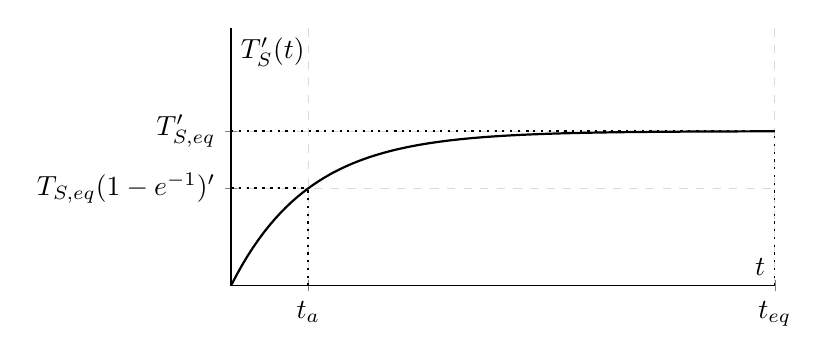
\begin{tikzpicture}
        \begin{axis}[
            xlabel=$t$,
            ylabel=$T_S'(t)$,
            xmin=0, xmax=7,
            ymin=0, ymax=5,
            xtick={0.994, 7},
            ytick={1.89, 3},
            yticklabels={$T_{S,eq} (1 - e^{-1})'$, $T_{S,eq}'$},
            xticklabels={$t_a$, $t_{eq}$},
            axis lines=middle,
            axis line style={-},
            width=0.7\textwidth,
            height=0.4\textwidth,
            grid=major,
            grid style={dashed, gray!30},
            % legend pos=north east,
            % legend style={font=\small, cells={align=left}},
            % legend cell align={left},
        ]
        \addplot[domain=0:7, black, thick,samples=100] {3*(1-exp(-x))};
        
        \addplot[domain=0:0.994, black, thick, dotted, samples=100] {3*0.63};
        \addplot[black, thick, dotted] coordinates {(0.994, 0) (0.994, 3*0.63)};
        % \node at (axis cs: 0.994, 3*0.63) [anchor=north west] {$T_{S,eq} (1-e^{-1})'$};
        % \node at (axis cs: 0.994, 0) [anchor=north] {$t_a$};

        \addplot[domain=0:7, black, thick, dotted, samples=100] {3};
        \addplot[black, thick, dotted] coordinates {(7, 0) (7, 3)};
        % \node at (axis cs: 3.5, 3) [anchor=south] {$T_{S,eq}'$};
        % \node at (axis cs: 7, 0) [anchor=north] {$t_{eq}$};

        \end{axis}
    \end{tikzpicture}
    \caption{Surface temperature change over time for the weak oceanic circulation}
    \label{fig:surface_temp_weak}
\end{figure}

\begin{tcolorbox}
    \textbf{Order-of-Magnitude Estimates:}\\
    We have expressions for $t_a$ and $T_{S,eq}'$ as follows:
    \begin{equation}
        t_a = \frac{m_{UO}c_O}{4\pi R_E^2 \gamma_{BB}} \quad \quad \text{and}
        \quad \quad T_{S,eq}' = \frac{\Delta Q_{EXT}}{\gamma_{BB}} \nonumber
    \end{equation}
    and we can use these to obtain some order-of-magnitude estimates. We use the
    following values:
    \begin{itemize}
        \item $m_{UO} = 3.4 \times 10^{19}\ \text{kg}$
        \item $c_O = 4.2 \times 10^3\ \text{J kg}^{-1} \text{K}^{-1}$
        \item $R_E = 6.4 \times 10^6\ \text{m}$
        \item $\gamma_{BB} = 4\epsilon' \sigma T_{S,eq}^3 \approx 3.8 
        \text{W m}^{-2} \text{K}^{-1}$
        \item $\Delta Q_{EXT} \approx 4\text{ W m}^{-2}$
    \end{itemize}

    \noindent From which we obtain:
    \begin{equation}
        t_a \approx 2.3\ \text{years} \quad \quad \text{and}
        \quad \quad T_{S,eq}' \approx 1\ \text{K} \nonumber
    \end{equation}

\end{tcolorbox}

\subsubsection{Strong Oceanic Circulation ($\eta \gg 1$)}
\label{sec:strong-oceanic-circulation}

In this case the upper and lower oceanic layers are strongly coupled, so we say
that $T_{DO}'(t) \approx T_S'(t)$ and therefore the second blue term in the 
equation cancels out. Once again, the equation be comes a first order linear
DE:
$$
\frac{dT_S'(t)}{dt} + \frac{4\pi R_E^2 \gamma_{BB}}{(m_{UO} + m_{DO})c_O} T_S'(t)
= \frac{4\pi R_E^2 \Delta Q_{EXT}(t)}{(m_{UO} + m_{DO})c_O}
$$

The solution, just as before is exponsential and we can write for $t_a$:
$$
\boxed{t_a = \frac{(m_{UO} + m_{DO})c_O}{4\pi R_E^2 \gamma_{BB}} \approx 
\frac{m_{DO}c_O}{4\pi R_E^2 \gamma_{BB}}} \quad \sim 100\text{s years}
$$

So we can see that the interaction between the upper and lower oceanic layers
has a significant effect on the adjustment timescale, i.e. it is a significant
damping factor on the rate of change of $T_S'(t)$. This is shown in figure
\ref{fig:surface_temp_timescale}.


\begin{figure}[h!]
    \centering
    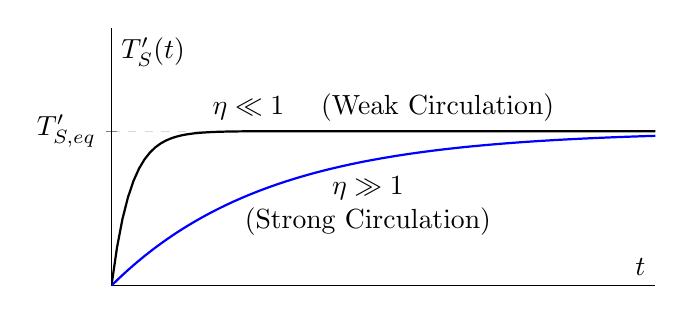
\begin{tikzpicture}
        \begin{axis}[
            xlabel=$t$,
            ylabel=$T_S'(t)$,
            xmin=0, xmax=7,
            ymin=0, ymax=5,
            xtick={0},
            ytick={3},
            yticklabels={$T_{S,eq}'$},
            xticklabels={},
            axis lines=middle,
            axis line style={-},
            width=0.7\textwidth,
            height=0.4\textwidth,
            grid=major,
            grid style={dashed, gray!30},
            legend pos=north east,
            legend style={font=\small, cells={align=left}},
            legend cell align={left},
        ]
        \addplot[domain=0:7, black, thick, samples=100] {3*(1-exp(-4*x))};
        \node at (axis cs: 3.5, 3) [anchor=south] 
        {$\eta \ll 1 \quad$ (Weak Circulation)};

        \addplot[domain=0:7, blue, thick, samples=100] {3*(1-exp(-0.5*x))};
        \node at (axis cs: 3.3, 2.3) [anchor=north, align=center] 
        {$\eta \gg 1$\\(Strong Circulation)};

        \end{axis}
    \end{tikzpicture}
    \caption{Strong vs weak oceanic circulation surface temperature change over time}
    \label{fig:surface_temp_timescale}
\end{figure}

\subsection{Climate Sensitivity}
\label{sec:climate-sensitivity}

In the section above (section \ref{sec:adjustment-timescale}) we have assumed a
number of things, some of which were not entirely realistic. 

One such assumption was the fact that no feedbacks other than blackbody feedback
were operating. We therefore used $\gamma_{BB}$ as the feedback parameter but in
fact we know that $\gamma = -\gamma_{BB} + \gamma_{\ce{H2O}} + 
\gamma_{\text{Albedo}} + \dots$ so we must rethink our model.We have seen that
$t_a \propto \frac{1}{\gamma}$ so it follows that changing $\gamma$ will change
the adjustment time $t_a$.\\

We define the \textbf{climate sensitivity} as the equillibrium global mean surface
temperature change in response to a doubling of \ce{CO2} concentration, i.e.
the previously seen $T_{S,eq}'$. To improve upon the previous blackbody-only
model, we can define the \textbf{net feedback parameter} $f$ as follows:
$$
f = \frac{\gamma_{\ce{H2O}} + \gamma_{\text{Albedo}} + \gamma_{\text{Clouds}} + 
\dots}{\gamma_{BB}} = \sum_i \frac{\gamma_i}{\gamma_{BB}}
$$
where $\gamma_i$ is the feedback parameter due to the $i$-th feedback process 
we wish to account for. We can now rewrite the climate sensitivity ($T_{S,eq}'$)
in terms of $f$ as follows:
$$
T_{S,eq}' = \frac{\Delta Q_{EXT}}{\gamma_{BB}} = \boxed{\frac{\Delta Q_{EXT}}{
\gamma_{BB} (1 - f)}}
$$
such that we now only have to consider the net feedback parameter $f$ to gain
insight into the \textbf{stability} of the climate system.\\

The following for some values of $f$ follow:
\begin{itemize}
    \item For negative values of $f$ (i.e. $f < 0$) the initial forcing $\Delta
    Q_{EXT}$ is dampened such that the adjustment time reduces and the equillibrium
    change in surface temperature is reduced. I.e. the equillibrium temperature
    is still higher than the initial temperature (because the 2x increase in \ce{CO2})
    is still present, but with a negative $f$ this increase in temperature is less
    than would be expected from the blackbody-only model.
    \item For $f = 0$ we essentially have the blackbody-only model.
    \item For positive values of $f$ (i.e. $f > 0$) the initial forcing $\Delta
    Q_{EXT}$ is amplified such that the adjustment time increases and the equillibrium
    change in surface temperature is increased. 
\end{itemize}

Finally, we notice that a value of $f = 1$ would mean that the climate system
is unable to reach an equillibrium, i.e. the planet is unable to ever radiate 
enough energy to space to counteract the effect of the original forcing and all
the operating feedbacks. This is called a \textbf{runaway greenhouse effect}.
